\documentclass[11pt]{article}
\usepackage[textwidth=18.0cm, textheight=23.0cm, top=2.0cm]{geometry}
\usepackage{pst-all}
\usepackage{amssymb}
\usepackage{tikz}
\usepackage{underscore}\begin{document}
\pagestyle{empty}


ClassName: \underline{\textbf{Class_03.2bp-6}}
\par
BinSize: \underline{\textbf{40 × 40}}
\par
ReduceSize: \underline{\textbf{40 × 40}}
\par
TypeNum: \underline{\textbf{20}}
\par
Num: \underline{\textbf{20}}
\par
OutS: \underline{\textbf{8000}}
\par
InS: \underline{\textbf{5447}}
\par
Rate: \underline{\textbf{0.681}}
\par
UB: \underline{\textbf{5}}
\par
LB0: \underline{\textbf{5}}
\par
LB: \underline{\textbf{5}}
\par
LBWithCut: \underline{\textbf{5}}
\par
NodeCut: \underline{\textbf{0}}
\par
ExtendedNodeCnt: \underline{\textbf{1}}
\par
GenNodeCnt: \underline{\textbf{1}}
\par
PrimalNode: \underline{\textbf{0}}
\par
ColumnCount: \underline{\textbf{5}}
\par
TotalCutCount: \underline{\textbf{0}}
\par
RootCutCount: \underline{\textbf{0}}
\par
LPSolverCnt: \underline{\textbf{1}}
\par
PricingSolverCnt: \underline{\textbf{0}}
\par
BranchAndBoundNum: \underline{\textbf{1}}
\par
isOpt: \underline{\textbf{true}}
\par
TimeOnInitSolution: \underline{\textbf{600.000 s}}
\par
TimeOnPrimal: \underline{\textbf{0.000 s}}
\par
TimeOnPricing: \underline{\textbf{0.000 s}}
\par
TimeOnRmp: \underline{\textbf{0.062 s}}
\par
TotalTime: \underline{\textbf{600.312 s}}
\par
\newpage


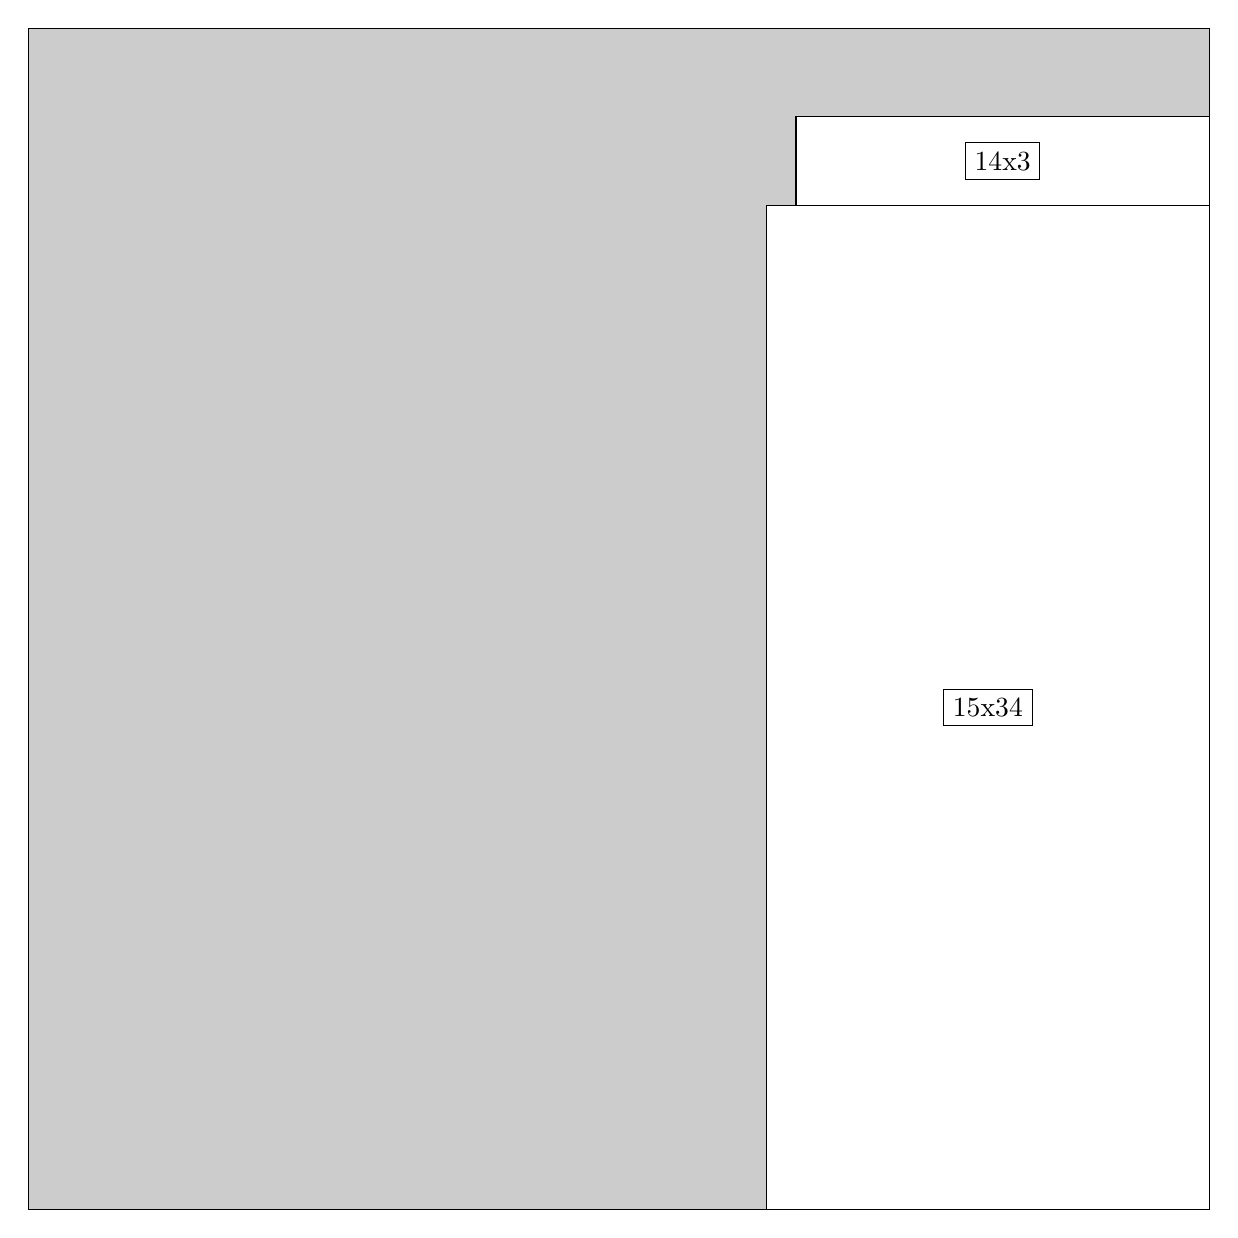
\begin{tikzpicture}[shorten >=1pt,scale=1.0,every node/.style={scale=1.0},->]
\tikzstyle{vertex}=[circle,fill=black!25,minimum size=14pt,inner sep=0pt]
\filldraw[fill=gray!40!white, draw=black] (0,0) rectangle (15.0,15.0);
\foreach \name/\x/\y/\w/\h in {15x34/9.375/0.0/5.625/12.75,14x3/9.75/12.75/5.25/1.125}
\filldraw[fill=white!40!white, draw=black] (\x,\y) rectangle node[draw] (\name) {\name} ++(\w,\h);
\end{tikzpicture}


w =15 , h =34 , x =25 , y =0 , v =510
\par
w =14 , h =3 , x =26 , y =34 , v =42
\par
\newpage


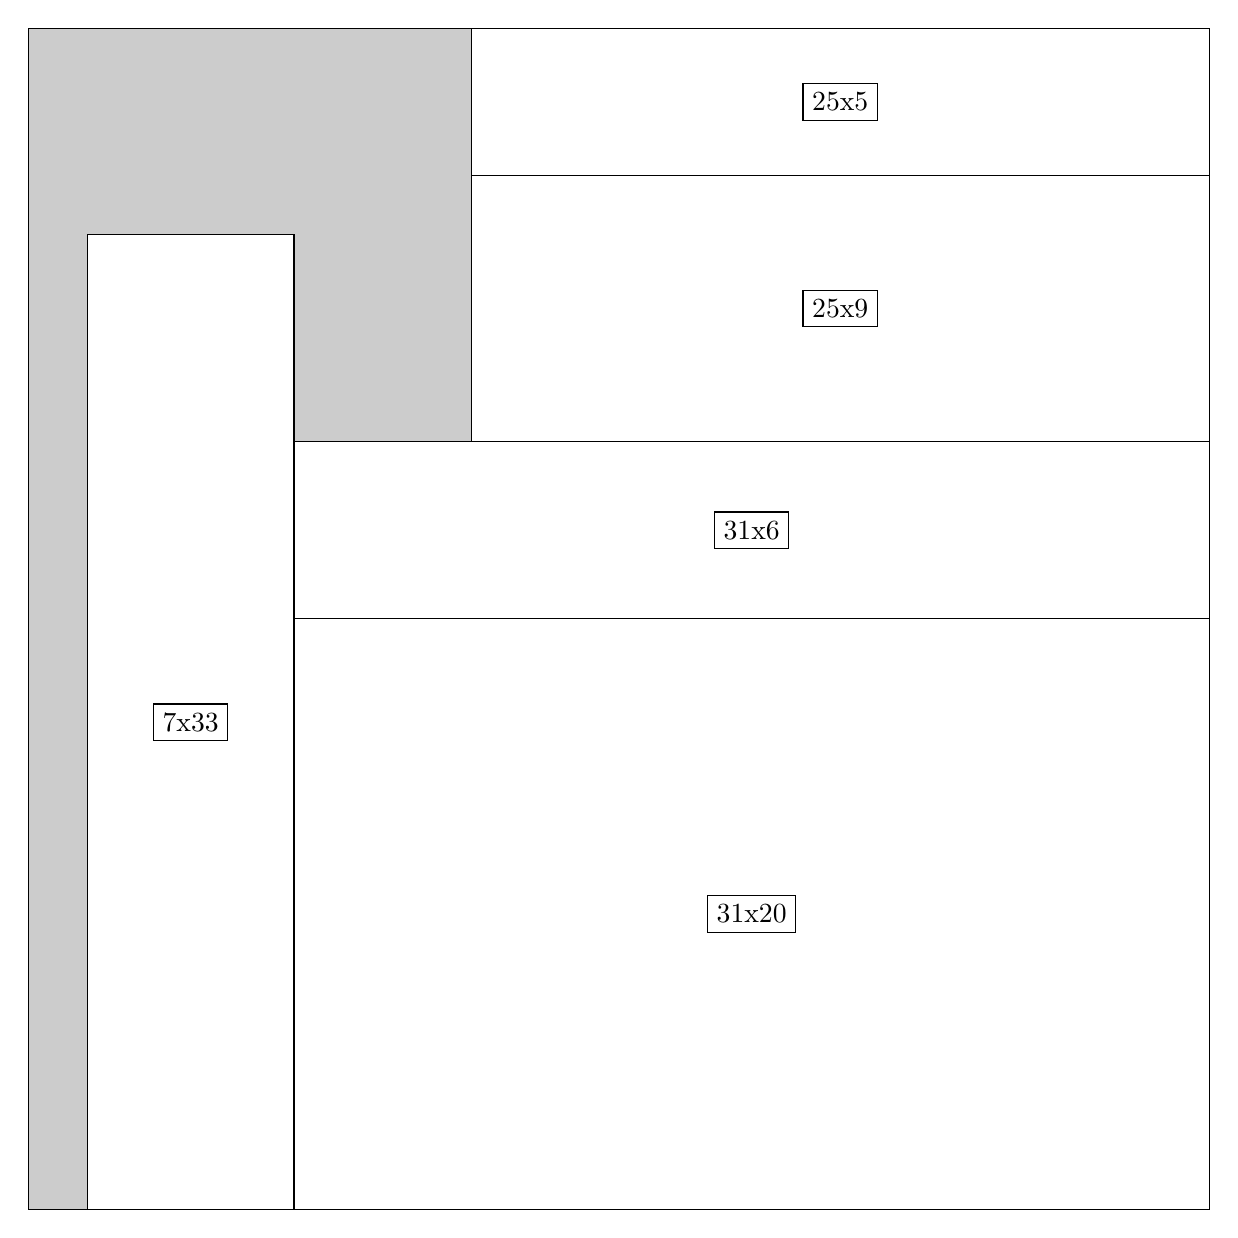
\begin{tikzpicture}[shorten >=1pt,scale=1.0,every node/.style={scale=1.0},->]
\tikzstyle{vertex}=[circle,fill=black!25,minimum size=14pt,inner sep=0pt]
\filldraw[fill=gray!40!white, draw=black] (0,0) rectangle (15.0,15.0);
\foreach \name/\x/\y/\w/\h in {31x20/3.375/0.0/11.625/7.5,31x6/3.375/7.5/11.625/2.25,25x9/5.625/9.75/9.375/3.375,25x5/5.625/13.125/9.375/1.875,7x33/0.75/0.0/2.625/12.375}
\filldraw[fill=white!40!white, draw=black] (\x,\y) rectangle node[draw] (\name) {\name} ++(\w,\h);
\end{tikzpicture}


w =31 , h =20 , x =9 , y =0 , v =620
\par
w =31 , h =6 , x =9 , y =20 , v =186
\par
w =25 , h =9 , x =15 , y =26 , v =225
\par
w =25 , h =5 , x =15 , y =35 , v =125
\par
w =7 , h =33 , x =2 , y =0 , v =231
\par
\newpage


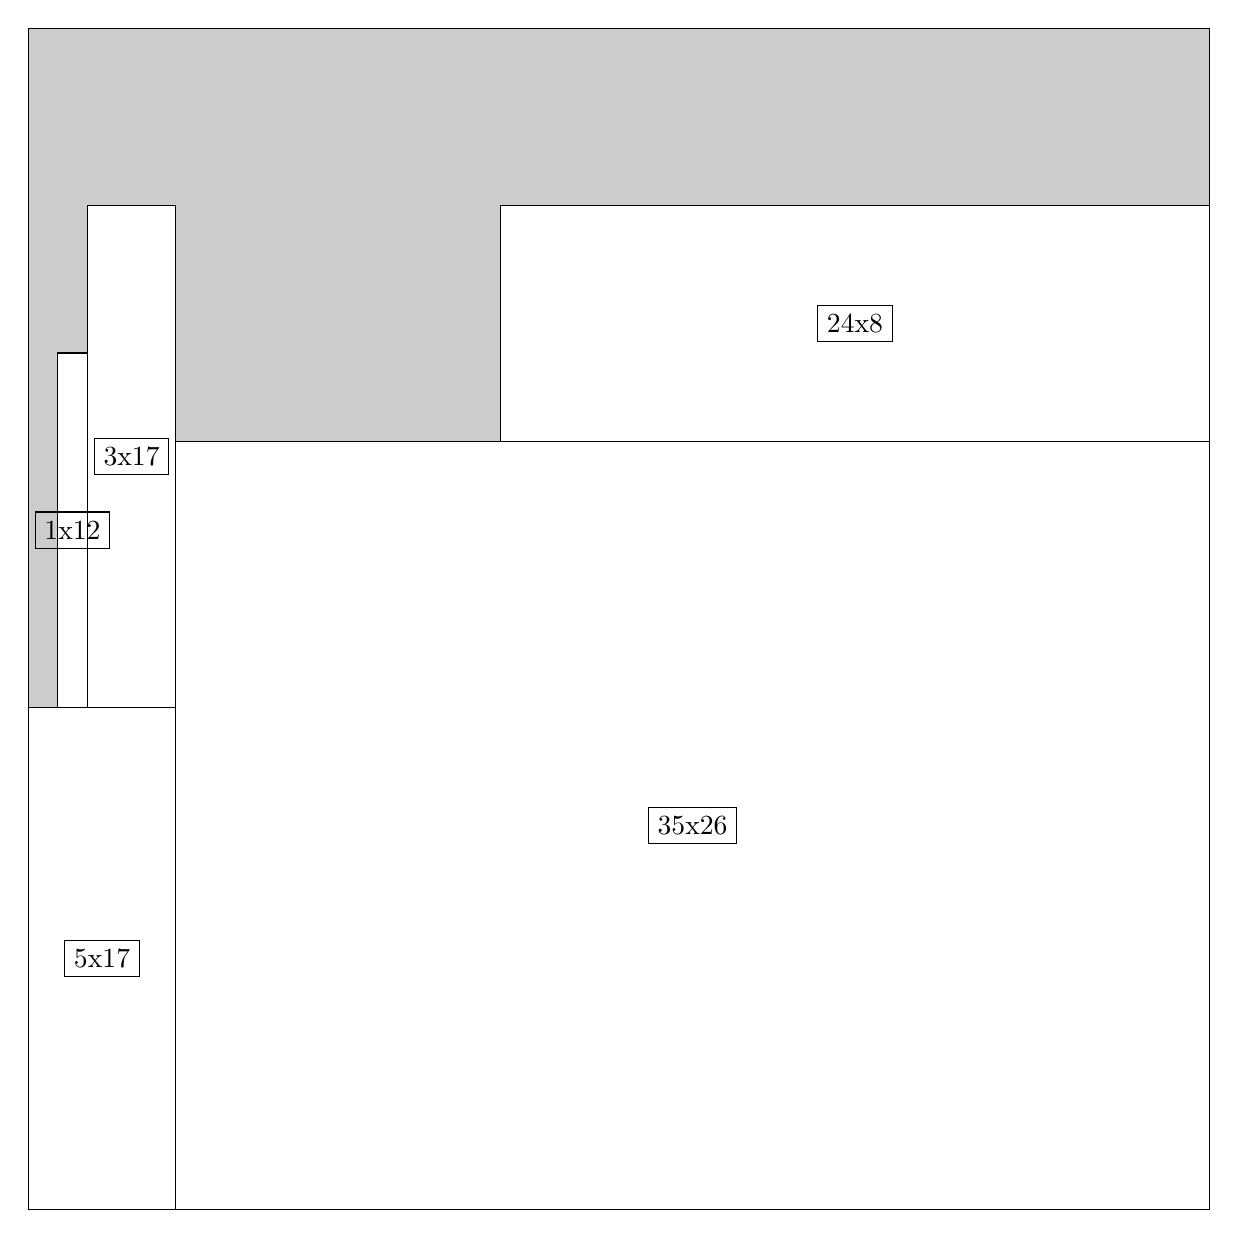
\begin{tikzpicture}[shorten >=1pt,scale=1.0,every node/.style={scale=1.0},->]
\tikzstyle{vertex}=[circle,fill=black!25,minimum size=14pt,inner sep=0pt]
\filldraw[fill=gray!40!white, draw=black] (0,0) rectangle (15.0,15.0);
\foreach \name/\x/\y/\w/\h in {35x26/1.875/0.0/13.125/9.75,24x8/6.0/9.75/9.0/3.0,5x17/0.0/0.0/1.875/6.375,3x17/0.75/6.375/1.125/6.375,1x12/0.375/6.375/0.375/4.5}
\filldraw[fill=white!40!white, draw=black] (\x,\y) rectangle node[draw] (\name) {\name} ++(\w,\h);
\end{tikzpicture}


w =35 , h =26 , x =5 , y =0 , v =910
\par
w =24 , h =8 , x =16 , y =26 , v =192
\par
w =5 , h =17 , x =0 , y =0 , v =85
\par
w =3 , h =17 , x =2 , y =17 , v =51
\par
w =1 , h =12 , x =1 , y =17 , v =12
\par
\newpage


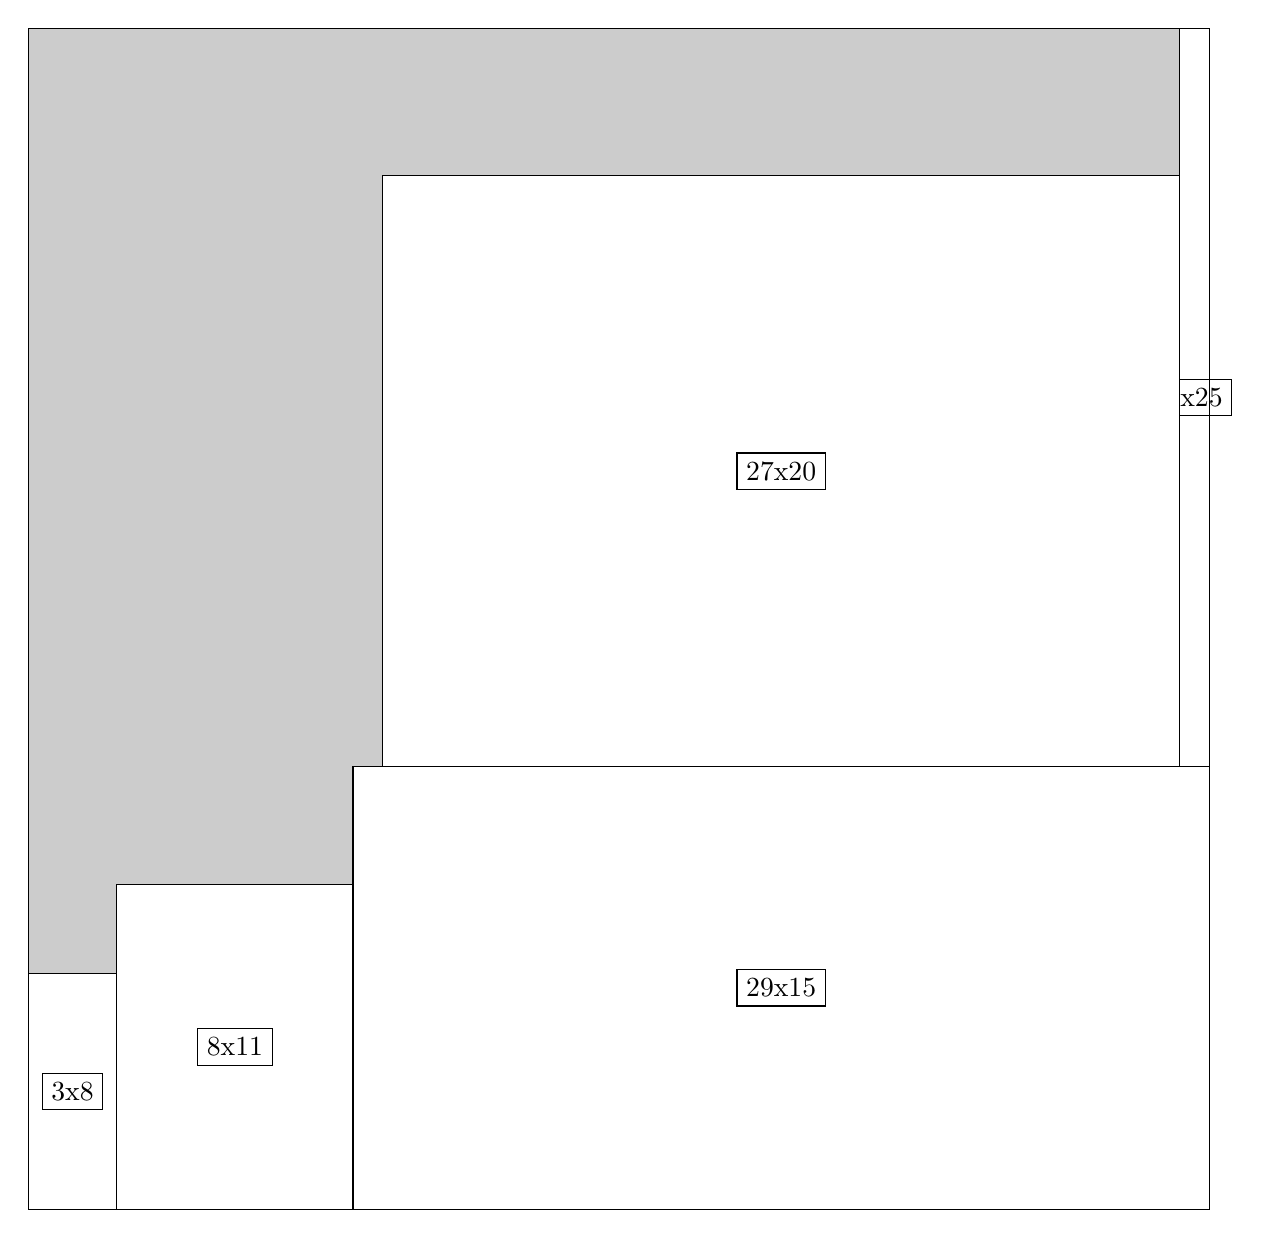
\begin{tikzpicture}[shorten >=1pt,scale=1.0,every node/.style={scale=1.0},->]
\tikzstyle{vertex}=[circle,fill=black!25,minimum size=14pt,inner sep=0pt]
\filldraw[fill=gray!40!white, draw=black] (0,0) rectangle (15.0,15.0);
\foreach \name/\x/\y/\w/\h in {29x15/4.125/0.0/10.875/5.625,1x25/14.625/5.625/0.375/9.375,27x20/4.5/5.625/10.125/7.5,8x11/1.125/0.0/3.0/4.125,3x8/0.0/0.0/1.125/3.0}
\filldraw[fill=white!40!white, draw=black] (\x,\y) rectangle node[draw] (\name) {\name} ++(\w,\h);
\end{tikzpicture}


w =29 , h =15 , x =11 , y =0 , v =435
\par
w =1 , h =25 , x =39 , y =15 , v =25
\par
w =27 , h =20 , x =12 , y =15 , v =540
\par
w =8 , h =11 , x =3 , y =0 , v =88
\par
w =3 , h =8 , x =0 , y =0 , v =24
\par
\newpage


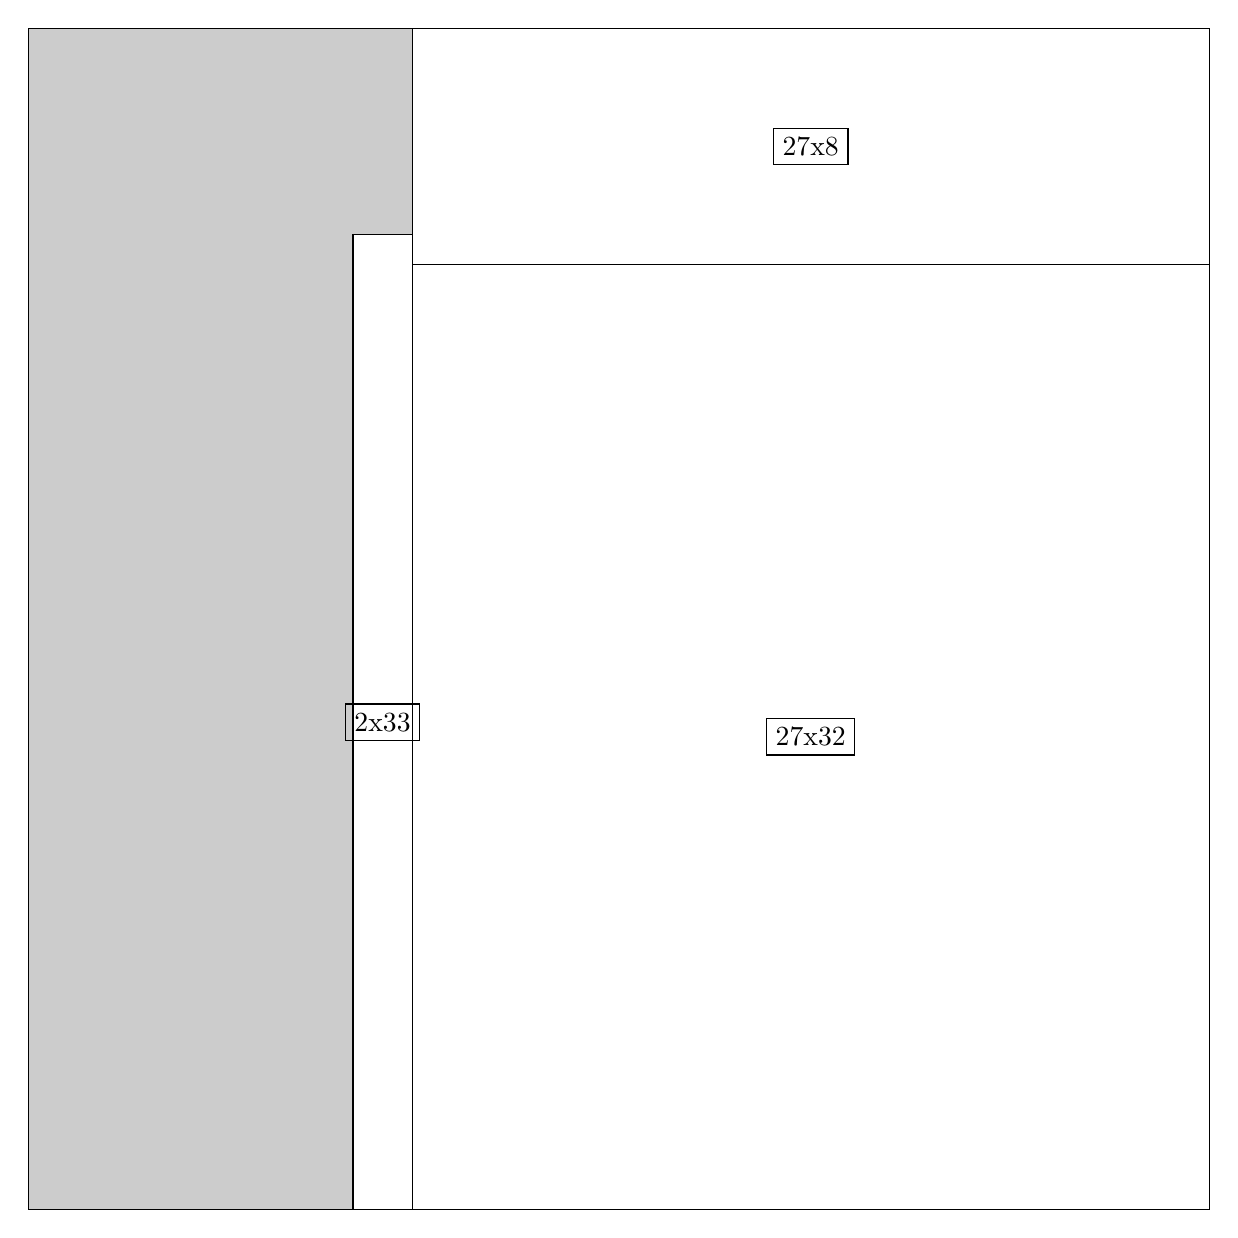
\begin{tikzpicture}[shorten >=1pt,scale=1.0,every node/.style={scale=1.0},->]
\tikzstyle{vertex}=[circle,fill=black!25,minimum size=14pt,inner sep=0pt]
\filldraw[fill=gray!40!white, draw=black] (0,0) rectangle (15.0,15.0);
\foreach \name/\x/\y/\w/\h in {27x32/4.875/0.0/10.125/12.0,27x8/4.875/12.0/10.125/3.0,2x33/4.125/0.0/0.75/12.375}
\filldraw[fill=white!40!white, draw=black] (\x,\y) rectangle node[draw] (\name) {\name} ++(\w,\h);
\end{tikzpicture}


w =27 , h =32 , x =13 , y =0 , v =864
\par
w =27 , h =8 , x =13 , y =32 , v =216
\par
w =2 , h =33 , x =11 , y =0 , v =66
\par
\newpage


\end{document}